\chapter{Technology of ice reservoirs}

This chapter describes the invention, evolution and construction methodology of AIR water storage technology.

\section{Invention of AIRs}

AIRs are a natural evolution of Ladakh's agricultural system. They can be related to traditional water
harvesting technologies like the zing, which are small tanks where meltwater is collected through the use of an
expensive and intricate network of channels. The mountain oases of the Hindu Kush and Karakoram ranges have
similar irrigation networks \citep{nusserLocalKnowledgeGlobal2016}.

\section{Evolution of AIRs}

Ice terraces are the oldest form of AIRs \citep{norphelArtificialGlacierHigh2009}. They used these irrigation
networks to amass a seasonal stock of ice by exploiting gravity and freezing winter temperatures. These
structures were built on south-facing slopes as a cascading series of rock walls in the river beds to reduce
runoff velocity and guide meltwater into shadowed areas (see Fig. \ref{fig:AIRforms}). The resulting shallow
pools begin to freeze as temperatures drop in winter, and ice accumulates. These AIRs are constructed as close
to the villages as possible. Being at a lower altitude than the natural glaciers, AIRS begin melting in April,
providing irrigation just in time for the start of the agricultural season. Chewang Norphel, a well known
engineer of the Leh Nutrition Project, introduced this innovation of local technology to Ladakh in the 1980s and
1990s \citep{vinceGlacierMan2009}.

A typical Ice stupa just requires a fountain nozzle mounted on a supply pipeline. The water source is usually a
spring or a glacial stream. Due to the altitude difference between the pipeline input and fountain output, water
ejects from the fountain nozzle as droplets that eventually lose their energy and accumulate as ice.  The
fountain is manually activated during the winter nights and is raised, through addition of metal pipes, when
significant ice accumulates below.

\begin{figure}[t]
\centering
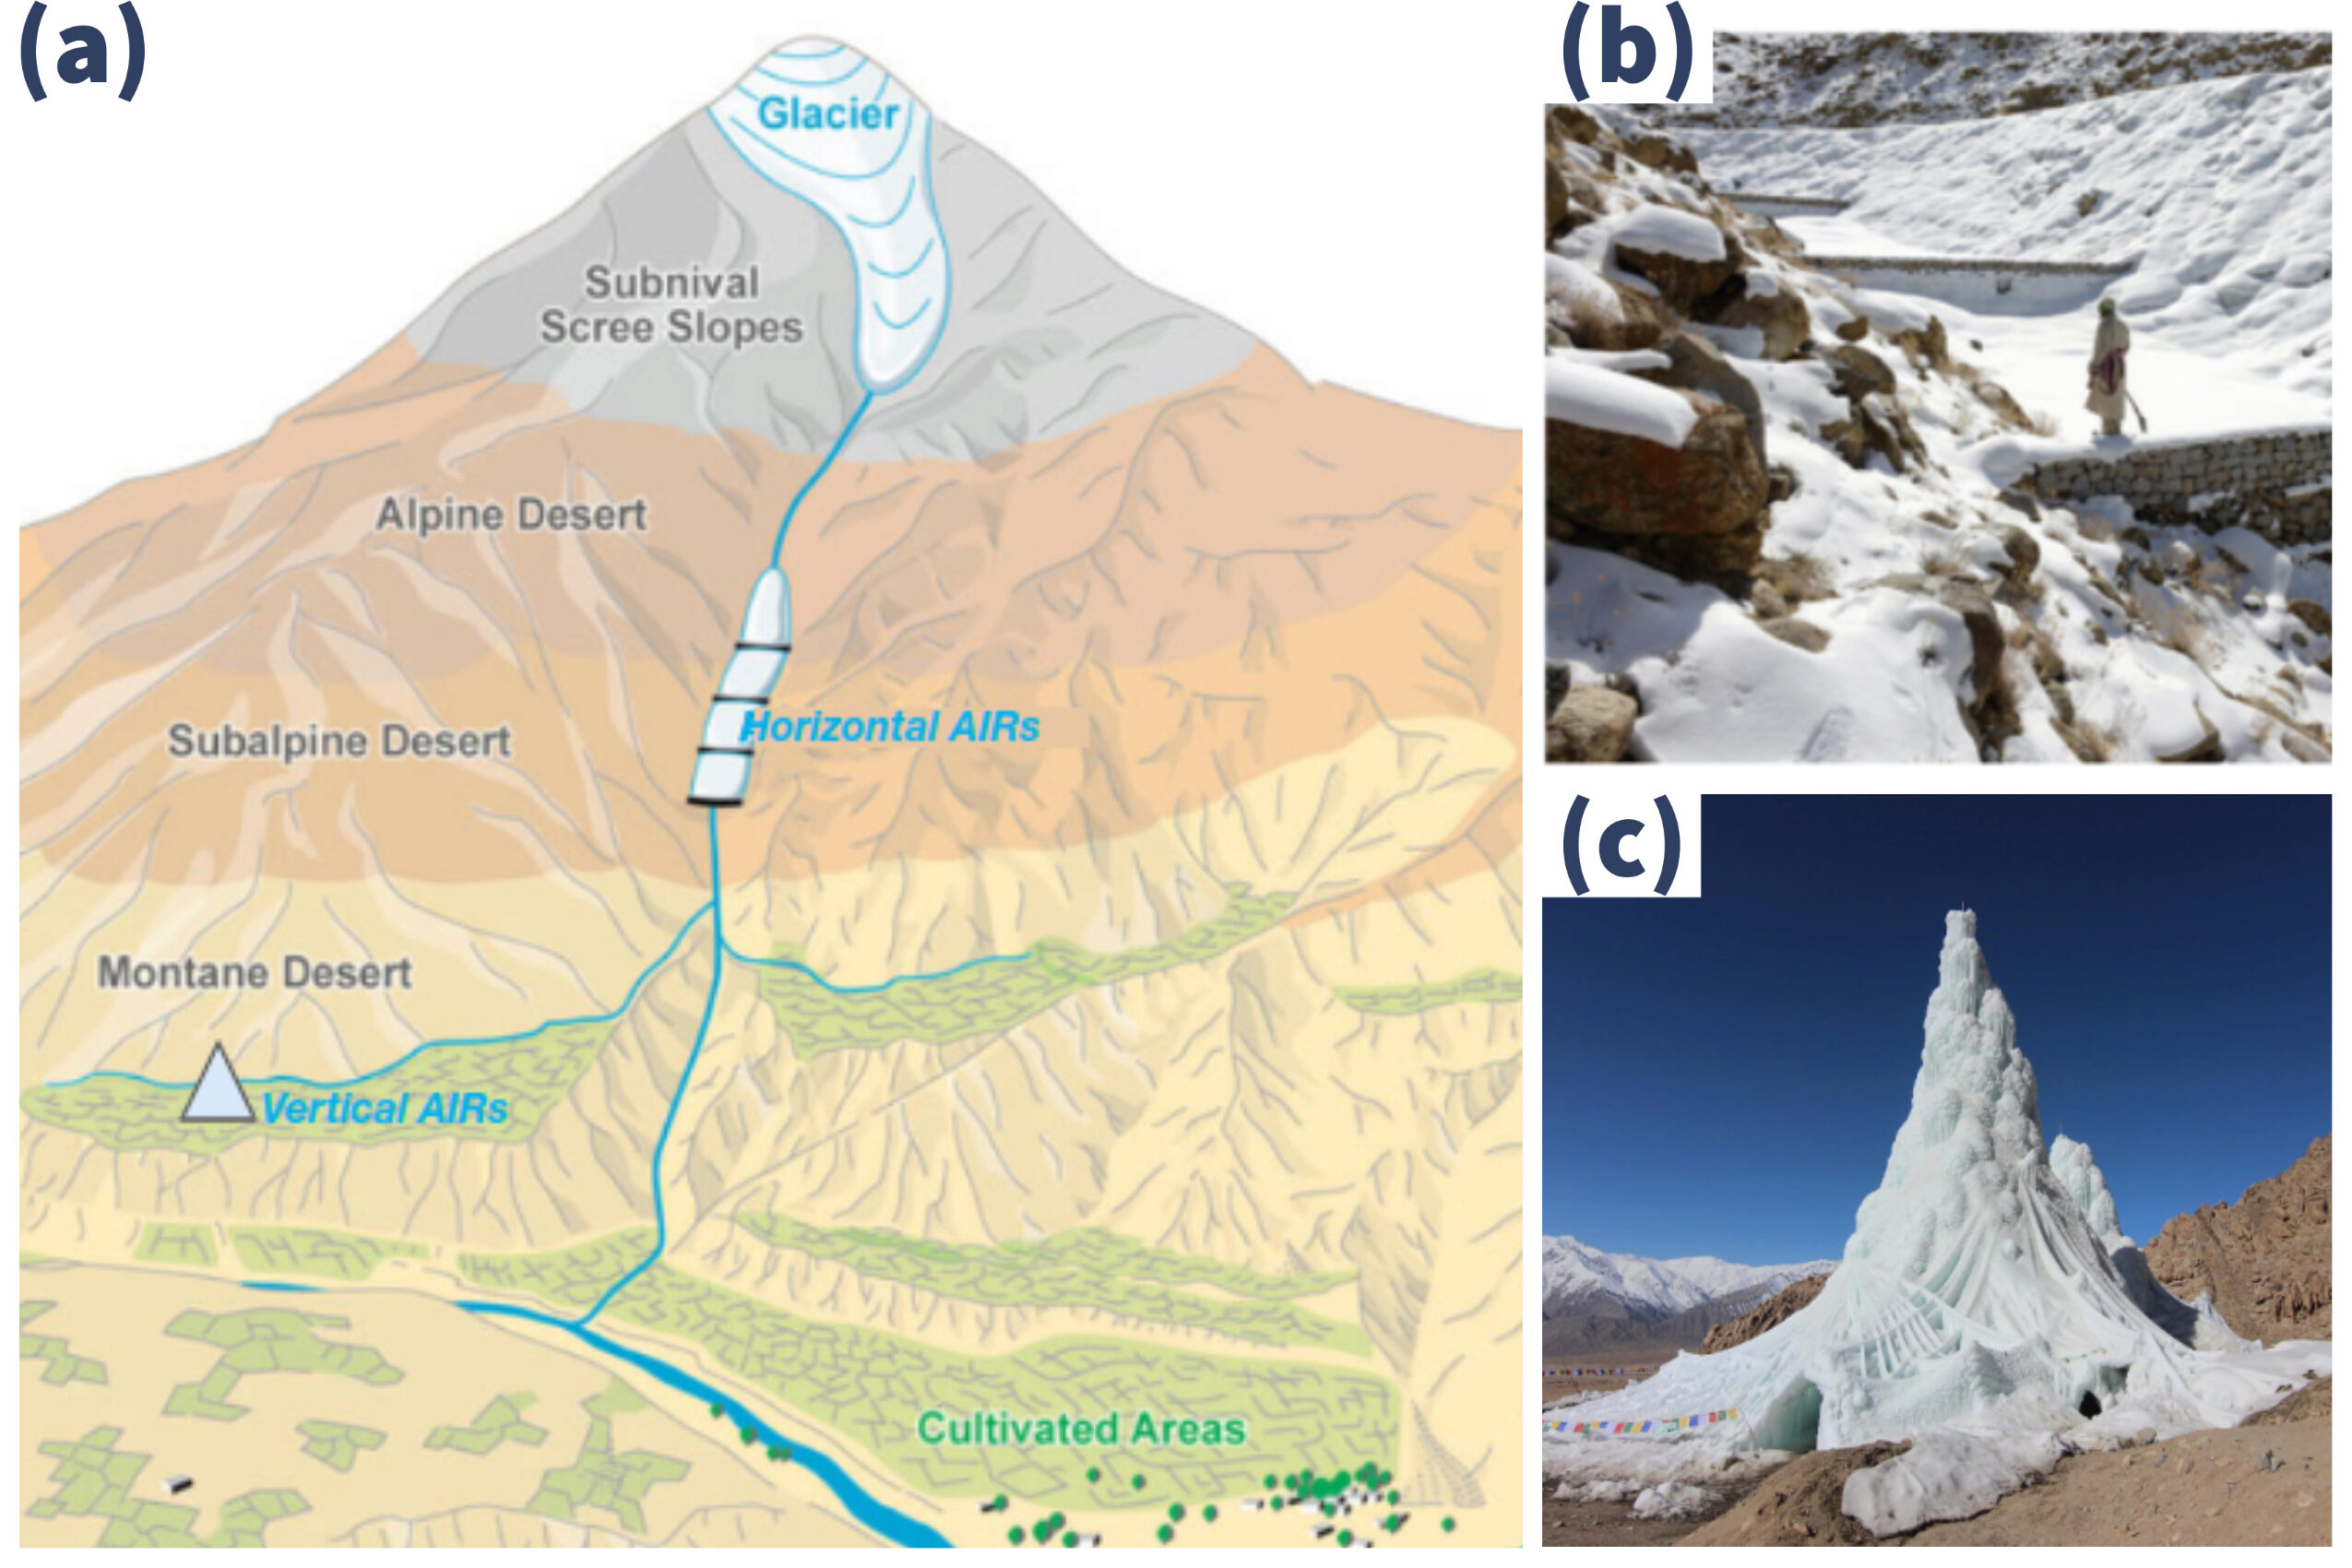
\includegraphics[width=12cm]{Figures/AIR_forms.jpg}

\caption{(a) Schematic overview of the position of artificial ice reservoirs. These constructions are located at
  altitudes between the glaciers and the irrigation networks in the cultivated areas. (b) Horizontal ice
  reservoirs at 3900 m, located above the village of Nang, Ladakh. The cascade is composed of a series of loose
  masonry walls ranging in height from 2 to 3 $m$, which help freeze water for storage. (c) Vertical ice
reservoirs at 3600 m, located above the village of Phyang, Ladakh. They are made using fountain systems. Adapted
from: \cite{nusserLocalKnowledgeGlobal2016}}

\label{fig:AIRforms}
\end{figure}
